\documentclass[12pt, letter]{article}

\usepackage{fullpage}
\usepackage{array}
\usepackage{enumitem}
\usepackage{mathtools}
\usepackage{graphicx}
\usepackage{caption}
\usepackage{float}
\usepackage{tikz}
\usetikzlibrary{automata, arrows}

\setlength{\parindent}{0cm}

\title{Assignment 3: Individual Full Design and Specification  \\ Job Search Tracking}
\author{William Richard}

\begin{document}
\maketitle

\section{Semantic Specification}

%\begin{description}
%\item[Function] 
%\item[Parameters]
%\item[Description]
%\item[Feedback]
%\item[Errors]
%\end{description}

%\hfill

\begin{description}
\item[Function] Recording information on objects
\item[Parameters] \hfill
\begin{enumerate} \item Object to be acted upon (person, company, etc) \item Information to be recorded (Name, address, etc) \end{enumerate}
\item[Description]
	An entry is either edited or created, with its fields populated by the information the user provides.  If relevant, new links are made between this object and other relevant objects (companies, jobs).
\item[Feedback] 	The user is shown a summary of the newly created/edited object, while highlighting the object on the graph.
\item[Errors] 	This should not cause errors - it is the action that the user will take many times in using this program, so it should be seamless and flawless as much as possible.
\end{description}

\hfill

\begin{description}
\item[Function] Specify custom object attributes 
\item[Parameters]\hfill \begin{enumerate} \item Object to add parameter to \item Custom parameter key \item Parameter value \end{enumerate}
\item[Description] 	Along with he automatic object attributes (name, address), the user is able to specify their own, custom attributes for any object.
\item[Feedback] The user is shown their custom parameter populated with the value they requested on a non-editable summary screen.
\item[Errors] \hfill \begin{enumerate} \item Key collision, if the user attempts to populate two attributes with the same key\end{enumerate}
\end{description}

\hfill


\begin{description}
\item[Function]  Specify object relationships
\item[Parameters] \hfill \begin{enumerate} \item Objects to create the relationship between (note and person relvant to the note, someone and their boss) \item Relationship name (note is about John Doe, Jane Doe is John Doe's boss) \end{enumerate}
\item[Description] 	The user is able to specify links between objects, for example a person works at a company for which an entry exists. There is a field that the user can fill in for each object for which such a relationship can exist.  The user fills in that field, possibly selecting a suggestion generated by the system.
\item[Feedback] A text block will be shown with the relationship name, and the revelvant object on the summary screen for the objects for which the relationship exists.  Perhaps a graph representation can also be created, showing objects as nodes and relationships as edges.
\item[Errors] \hfill \begin{enumerate} \item Object does not exist $\to$ user should be given the option to create the object. \end{enumerate}
\end{description}

\hfill

\section{Syntactic Specification}

\subsection{For each object (company, person, job, note)}

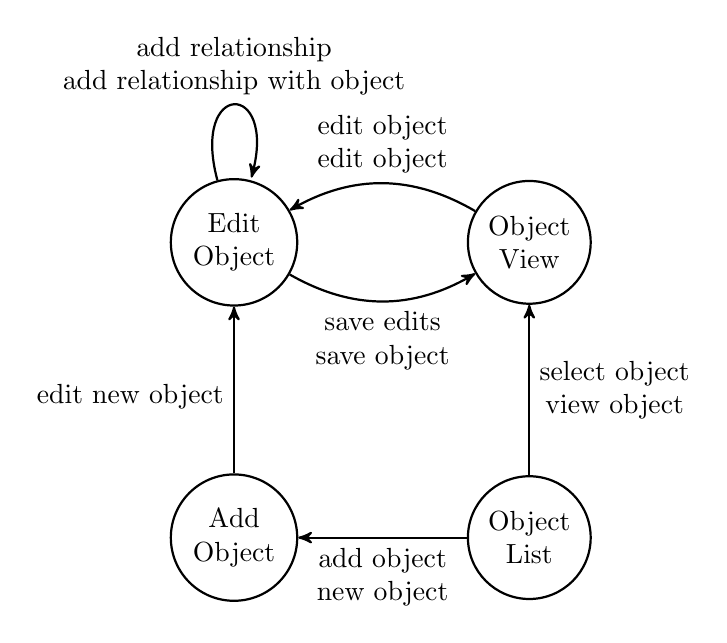
\begin{tikzpicture} [node distance=3.75cm, thick, align=center, ->,>=stealth']


\node[state] 	(object_list) 							{Object \\ List};
\node[state] 	(object_view)	[above of=object_list]	{Object \\ View};
\node[state]		(edit_object)		[left of=object_view]		{Edit \\ Object};
\node[state]		(add_object)		[left of=object_list]		{Add \\ Object};

\path[->]	(object_list)		edge			node	[right]		{select object \\ view object} 	(object_view)
					edge			node	[below]	{add object \\ new object}	(add_object)
		(object_view)	edge	[bend right]	node	[above] 	{edit object \\ edit object}		(edit_object)
		(edit_object)		edge	[bend right]	node	[below]	{save edits\\ save object}		(object_view)
					edge 	[loop above]	node	{add relationship \\ add relationship with object}	(edit_object)
		(add_object)	edge			node	[left]	{\\ edit new object}		(edit_object)
;

\end{tikzpicture}

\subsection{Transitions Between Object Lists}

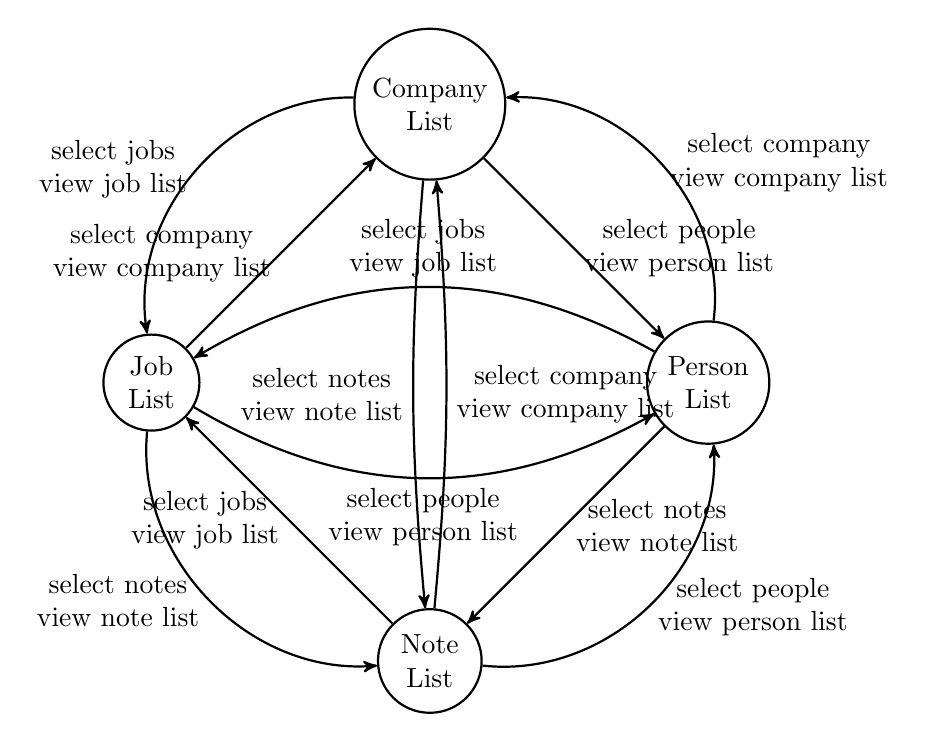
\begin{tikzpicture} [node distance=5cm, thick, align=center, ->,>=stealth']


\node[state] 	(company) 					{Company \\ List};
\node[state] 	(person)	[below right of=company]		{Person \\ List};
\node[state]		(job)		[below left of=company]	{Job \\ List};
\node[state]		(note)		[below right of=job]		{Note \\ List};

\path[->]
		(company)	edge		node	[right]	{select people \\ view person list}	(person)
				edge	[bend right=50]	node	[left]	{select jobs \\ view job list} 		(job)
				edge	[bend right=5]	node	[left]	{select notes \\ view note list}		(note)
		(person)	edge	[bend right=50]	node	[right]	{select company \\ view company list}	(company)
				edge	[bend right=30]	node	[above]	{select jobs \\ view job list} 		(job)
				edge		node	[right]	{select notes \\ view note list}		(note)
		(job)		edge		node	[left]	{select company \\ view company list}	(company)
				edge 	[bend right=30]	node	[below]	{select people \\ view person list}	(person)
				edge	[bend right=50]	node	[left]	{select notes \\ view note list}		(note)
		(note)		edge 	[bend right=50]	node	[right]	{select people \\ view person list}	(person)
				edge	[bend right=5]	node	[right]	{select company \\ view company list}	(company)
				edge		node	[left]	{select jobs \\ view job list} 		(job)
;

\end{tikzpicture}


\section{Lexical Design Specification}
\begin{tabular}[H]{|m{2.5cm} | m{15cm}|}
\hline
Token & System Operations \\
\hline
view object & Retrieve object attributes and display them on screen \\
edit object & Allow the user to edit object attributes, adding new ones if needed.  Do not save changes until confirmed by user.  \\
new object & Create a new object, immediately begin editing it.\\
save object & Save object and its attributes in the backend database.\\
add relationship & Save an object attribute, with the value being another object id. Like any other edit, only save changes after user confirms save.\\
view object list & Retrieve a list of objects of the specified type.  Display them, along with pertinent identifying information. \\
\hline

\end{tabular}

\section{Storyboard}

This storyboard depicts adding a new contact, along with their company - it was my second usage scenario from the previous assignment.

Note that boxes with a single edge are text boxes (like a form) while boxes with a double edge are buttons.  For example, in Figure \ref{fig2}, the squares along the top of the image are buttons, below that they are text boxes, until the save box at the button at the bottom right.

\begin{figure}[H]
\centering
\begin{minipage}[t]{.4\linewidth}
\centering
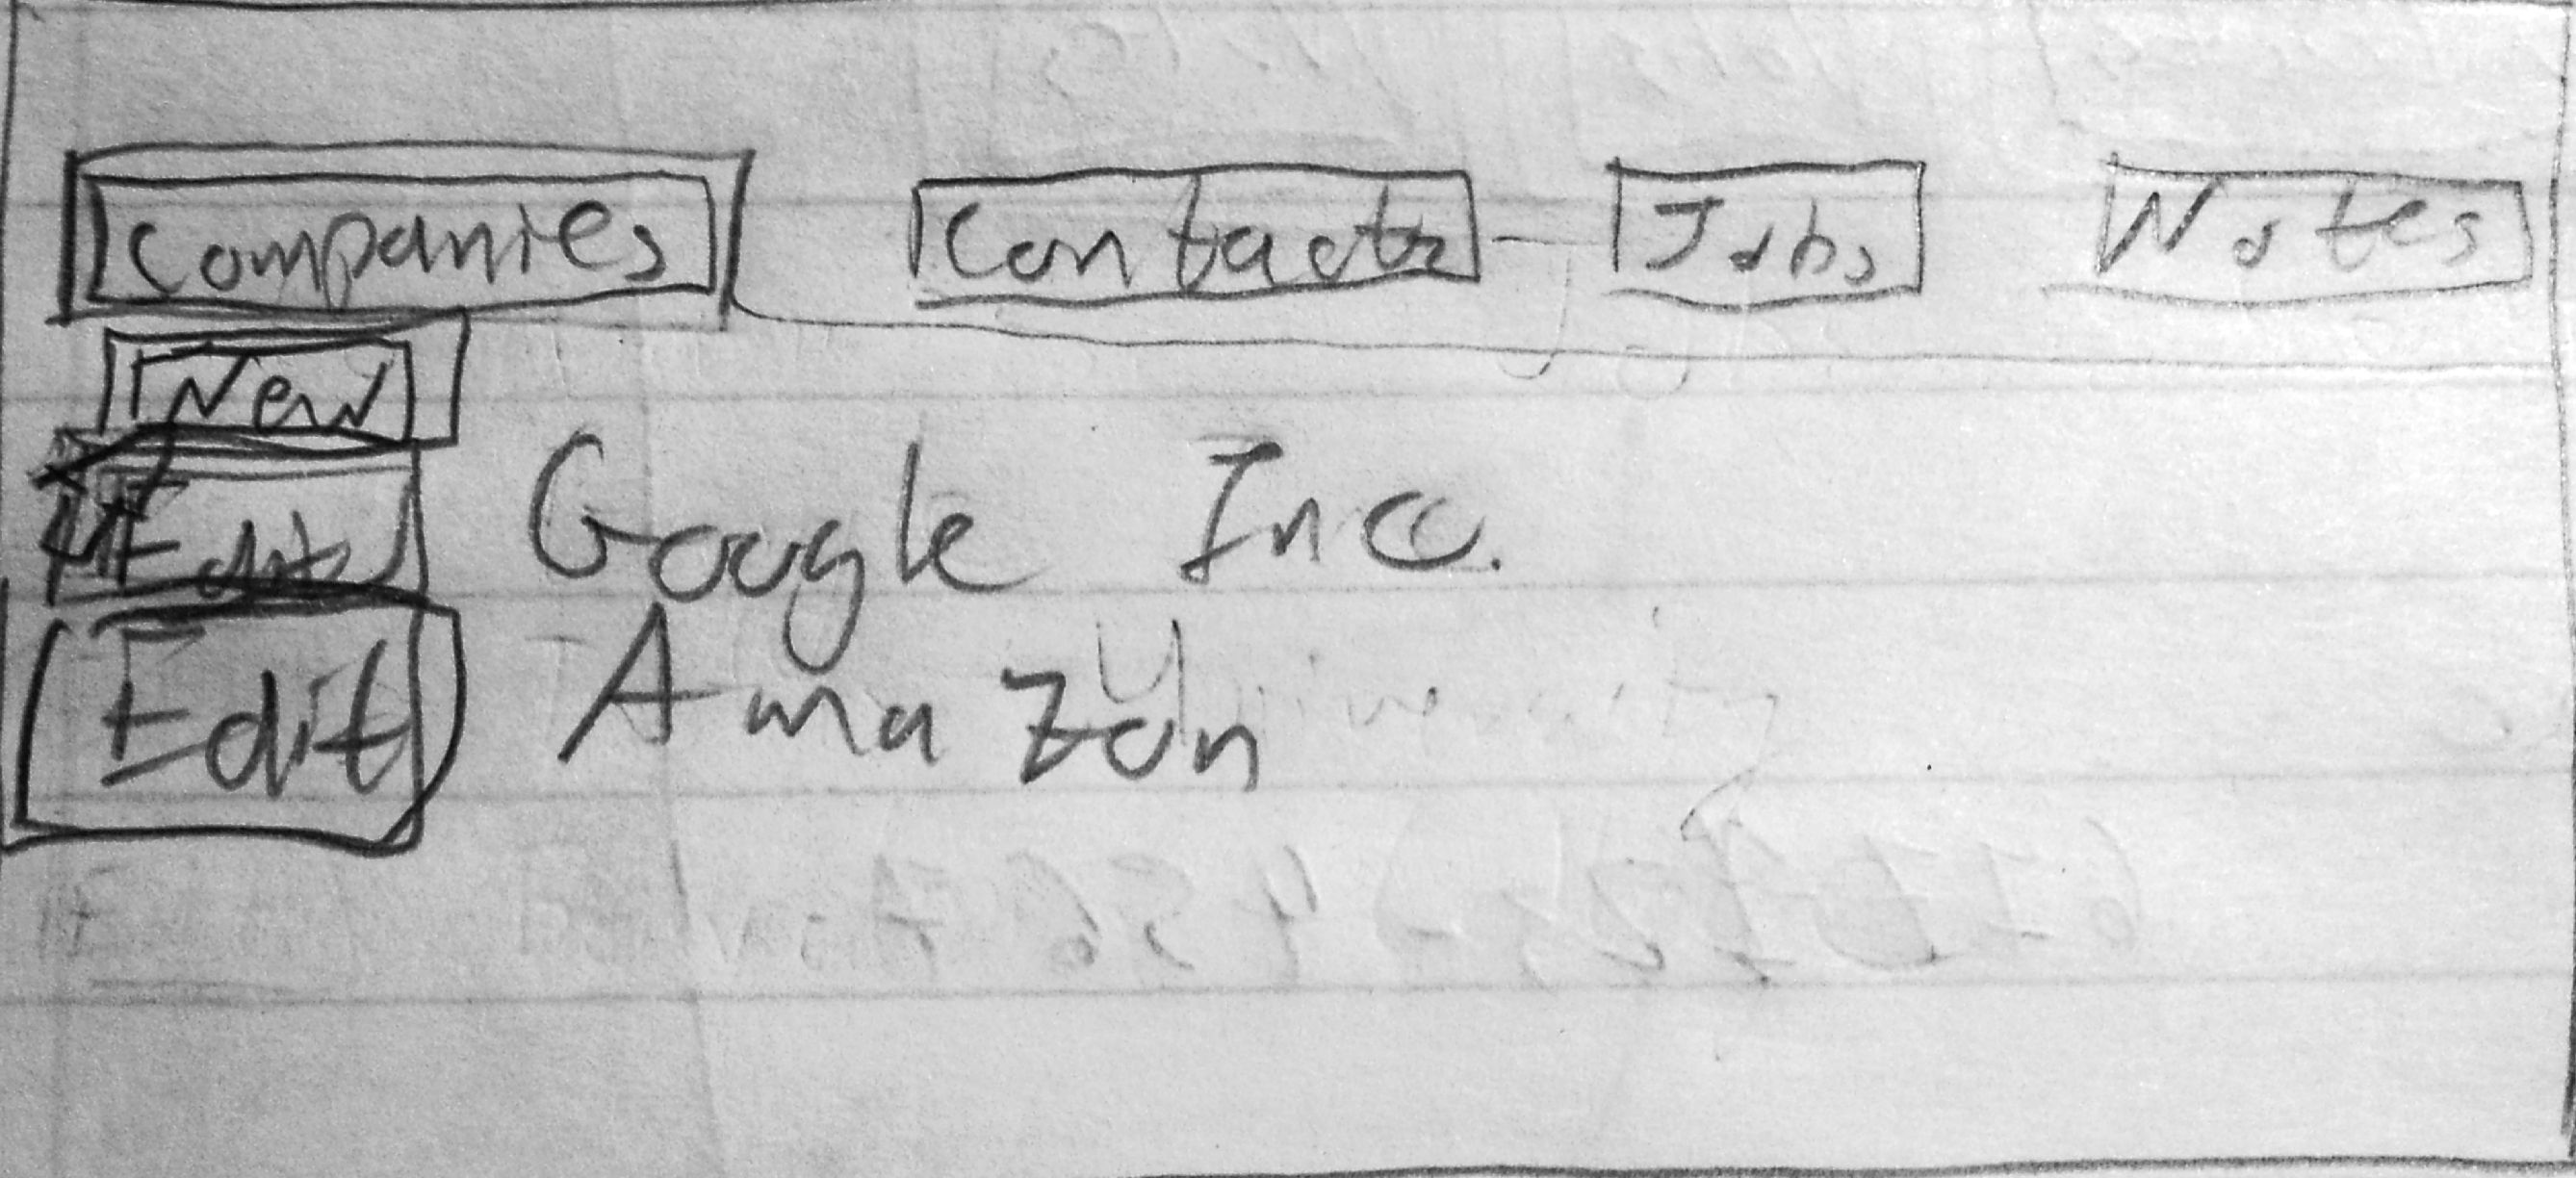
\includegraphics[width=\textwidth]{story_1.jpg}
\captionof{figure}{Starting at the company list page}
\end{minipage}
\hspace{.5cm}
\begin{minipage}[t]{.4\linewidth}
\centering
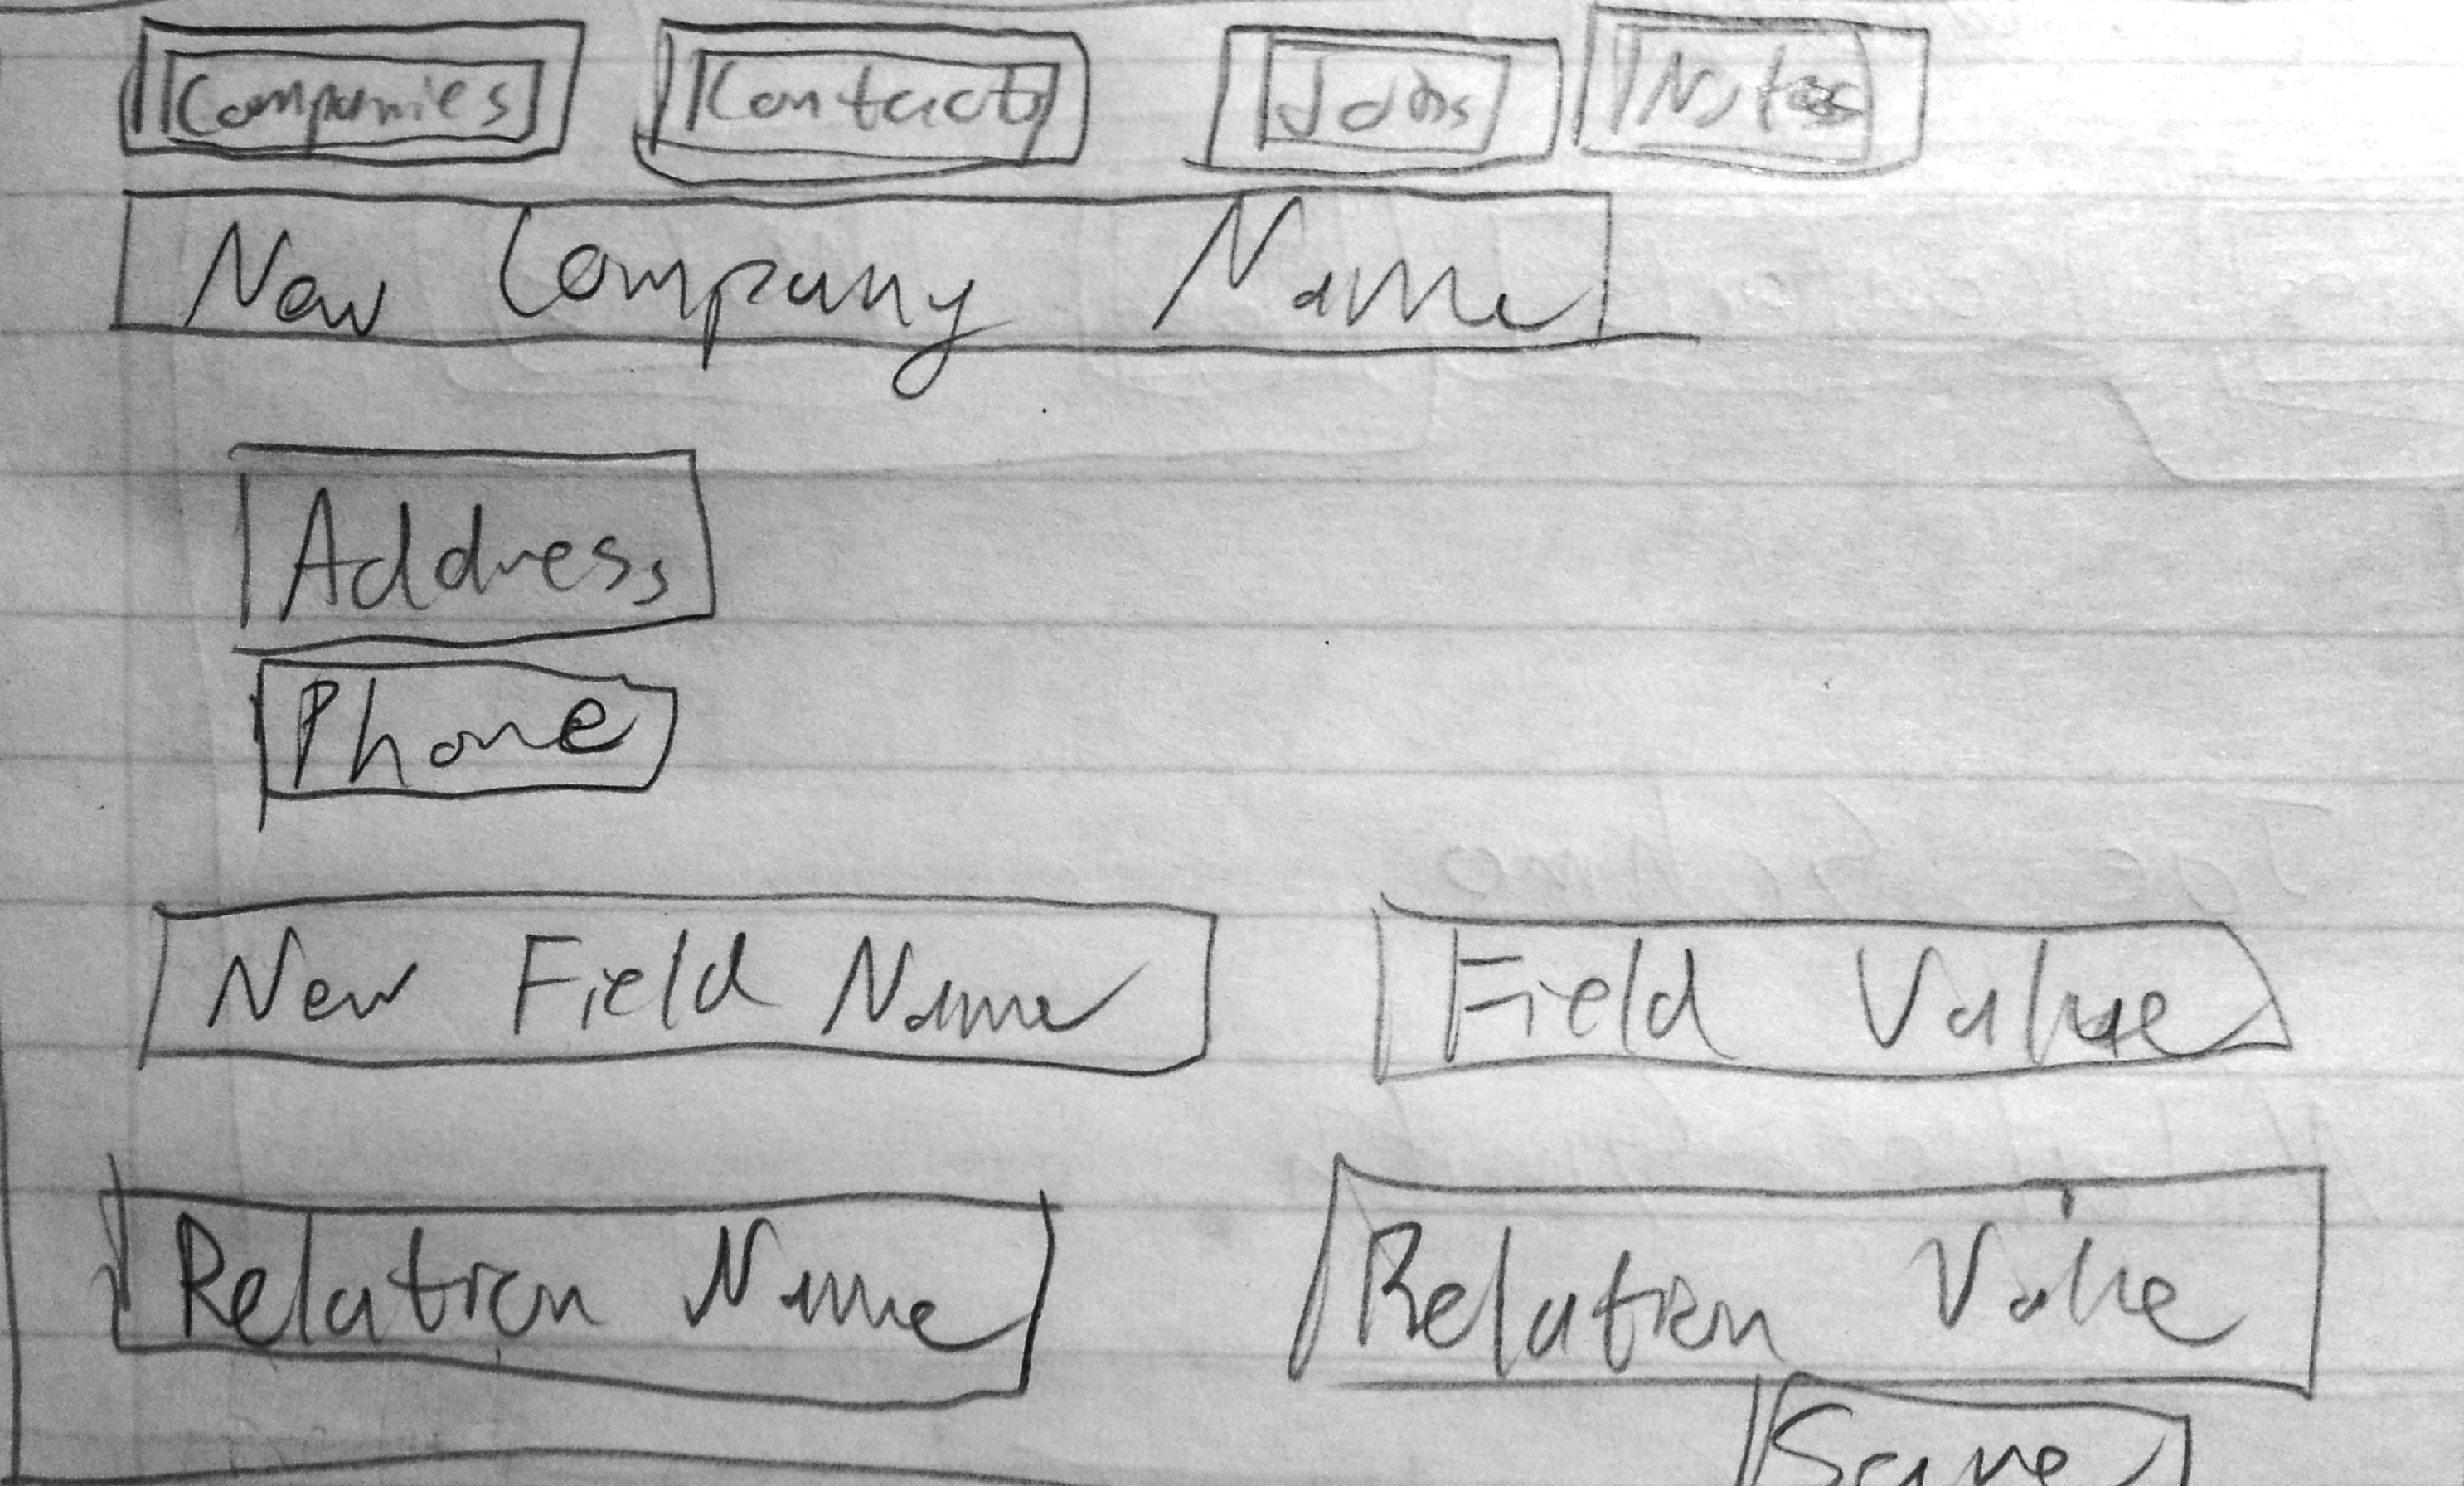
\includegraphics[width=\textwidth]{story_2.jpg}
\captionof{figure}{The blank new company page.}
\label{fig2}
\end{minipage}

\end{figure}

\begin{figure}[H]
\centering



\begin{minipage}[t]{.4\linewidth}
\centering
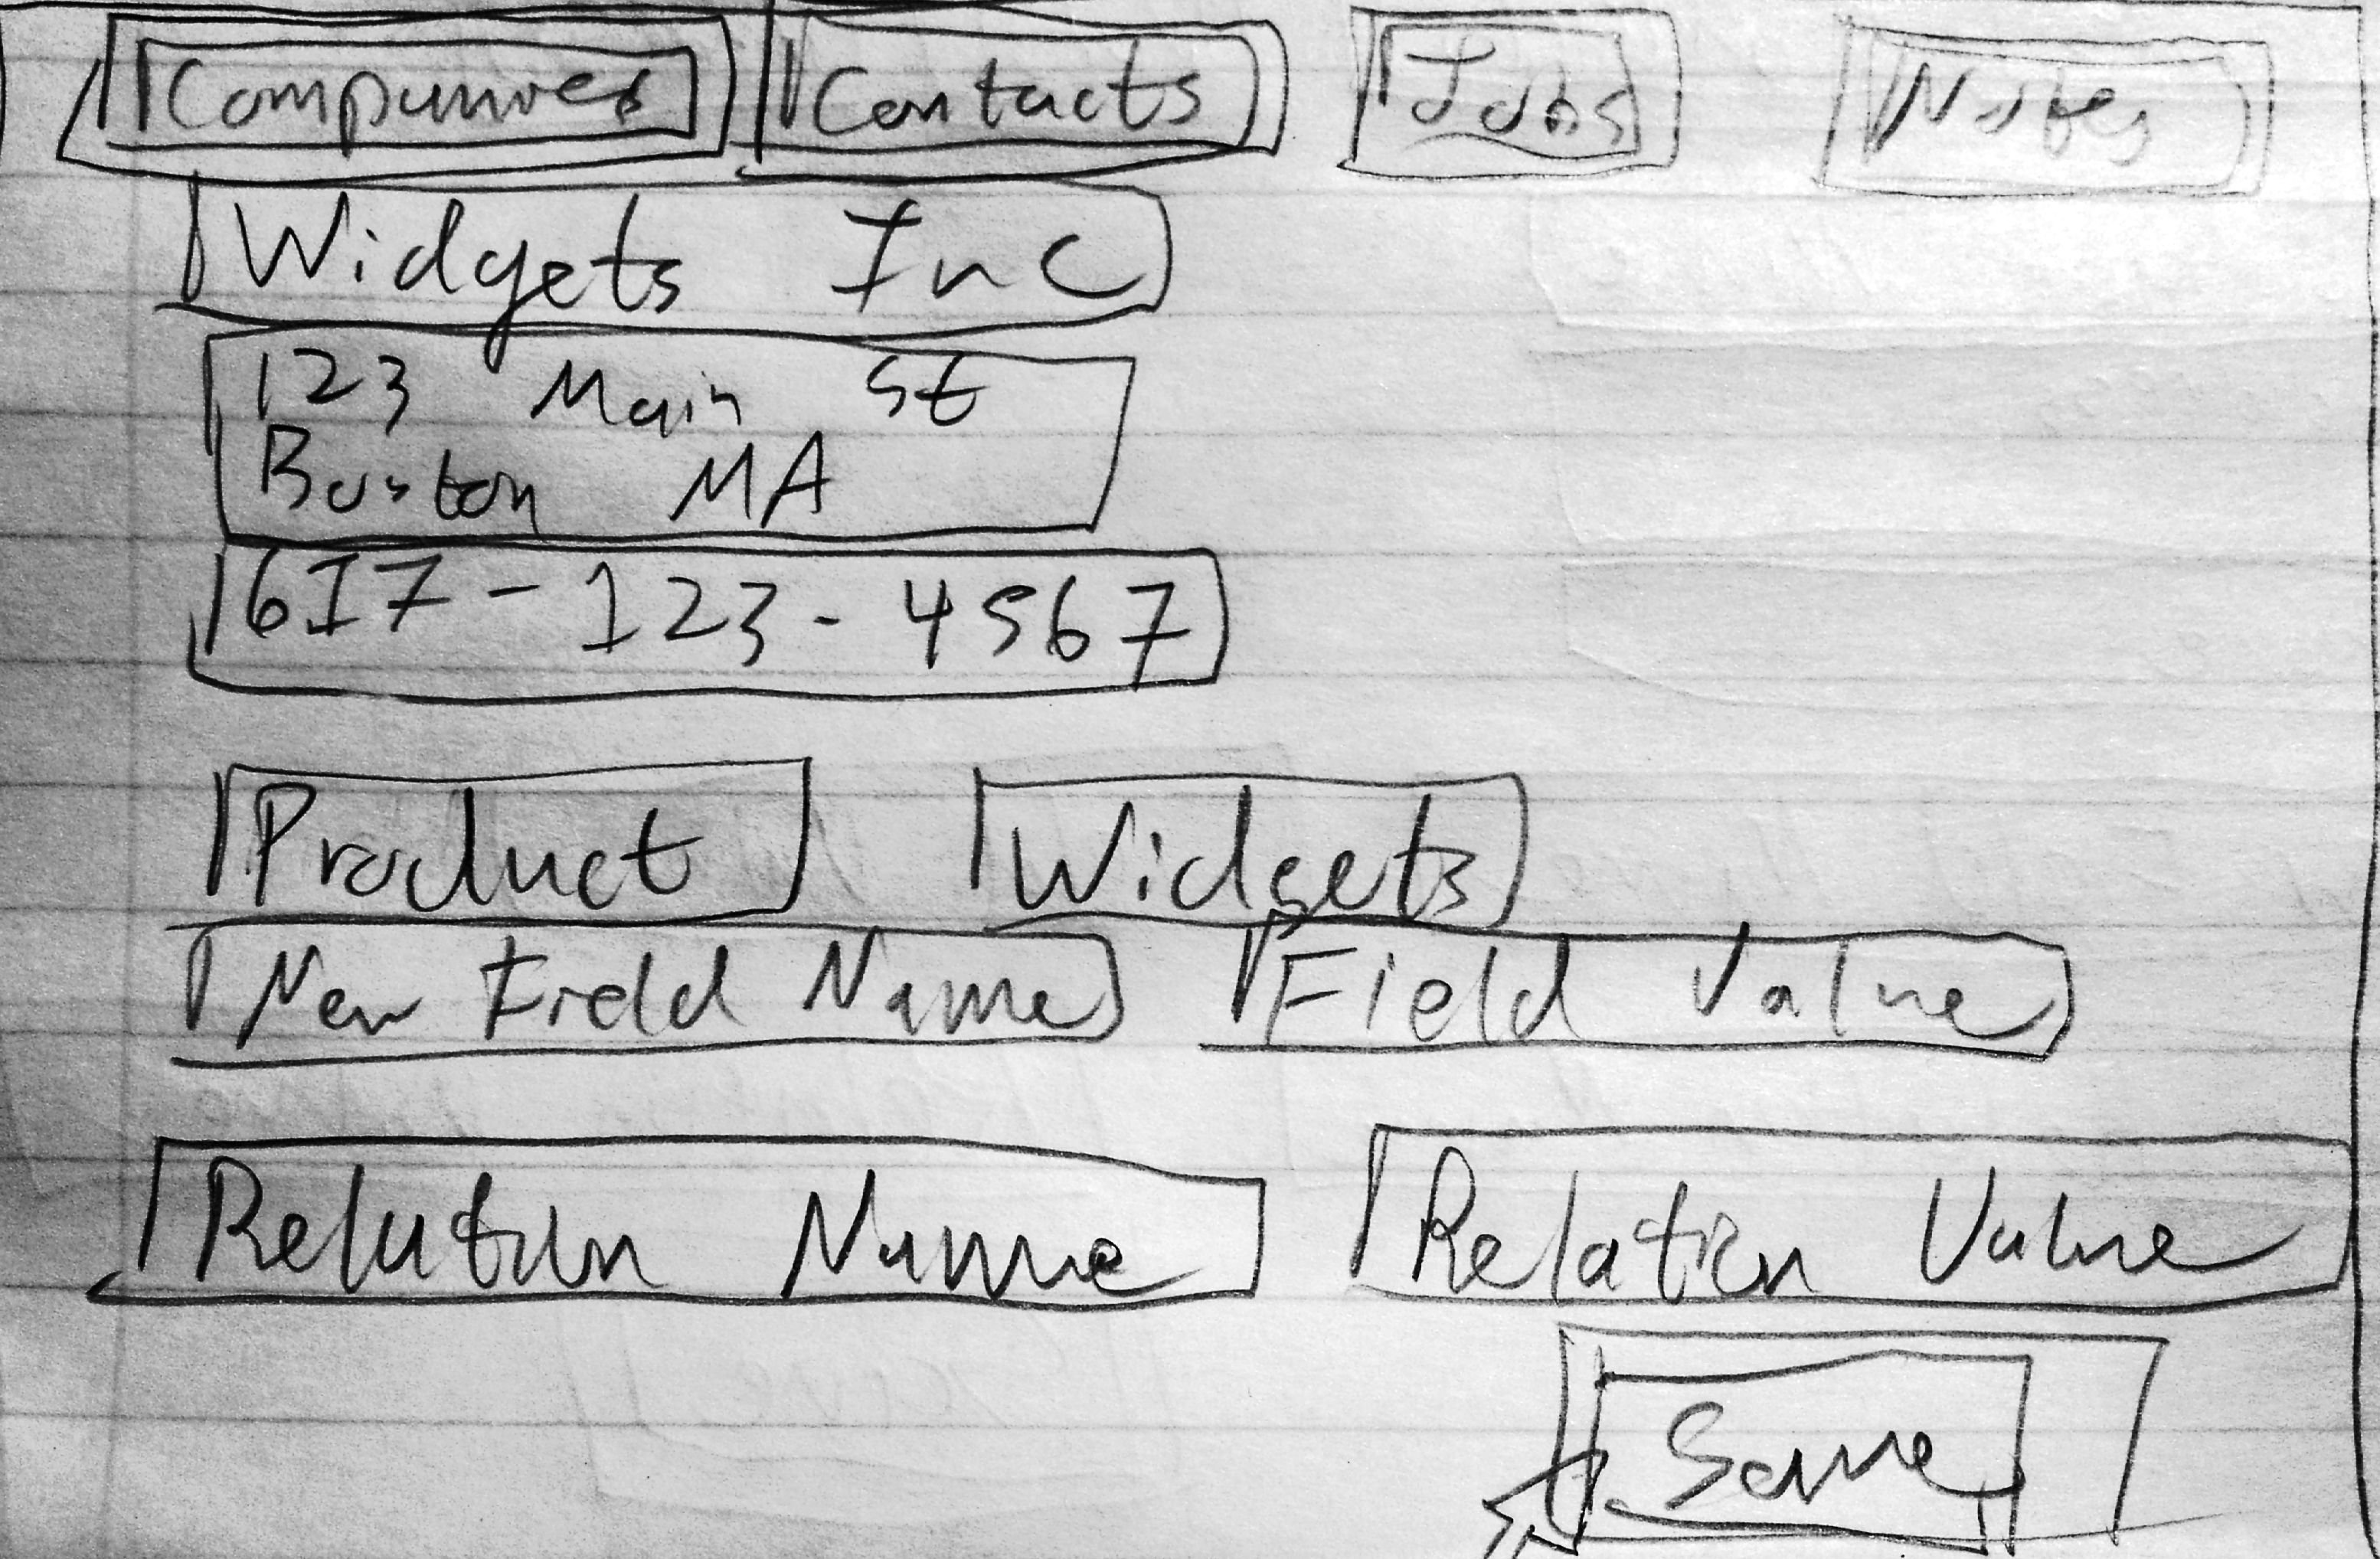
\includegraphics[width=\textwidth]{story_3.jpg}
\captionof{figure}{The new company, populated.  Notice the custom field 'Product' with the value 'Widgets'.}
\end{minipage}
\hspace{.5cm}
\begin{minipage}[t]{.4\linewidth}
\centering
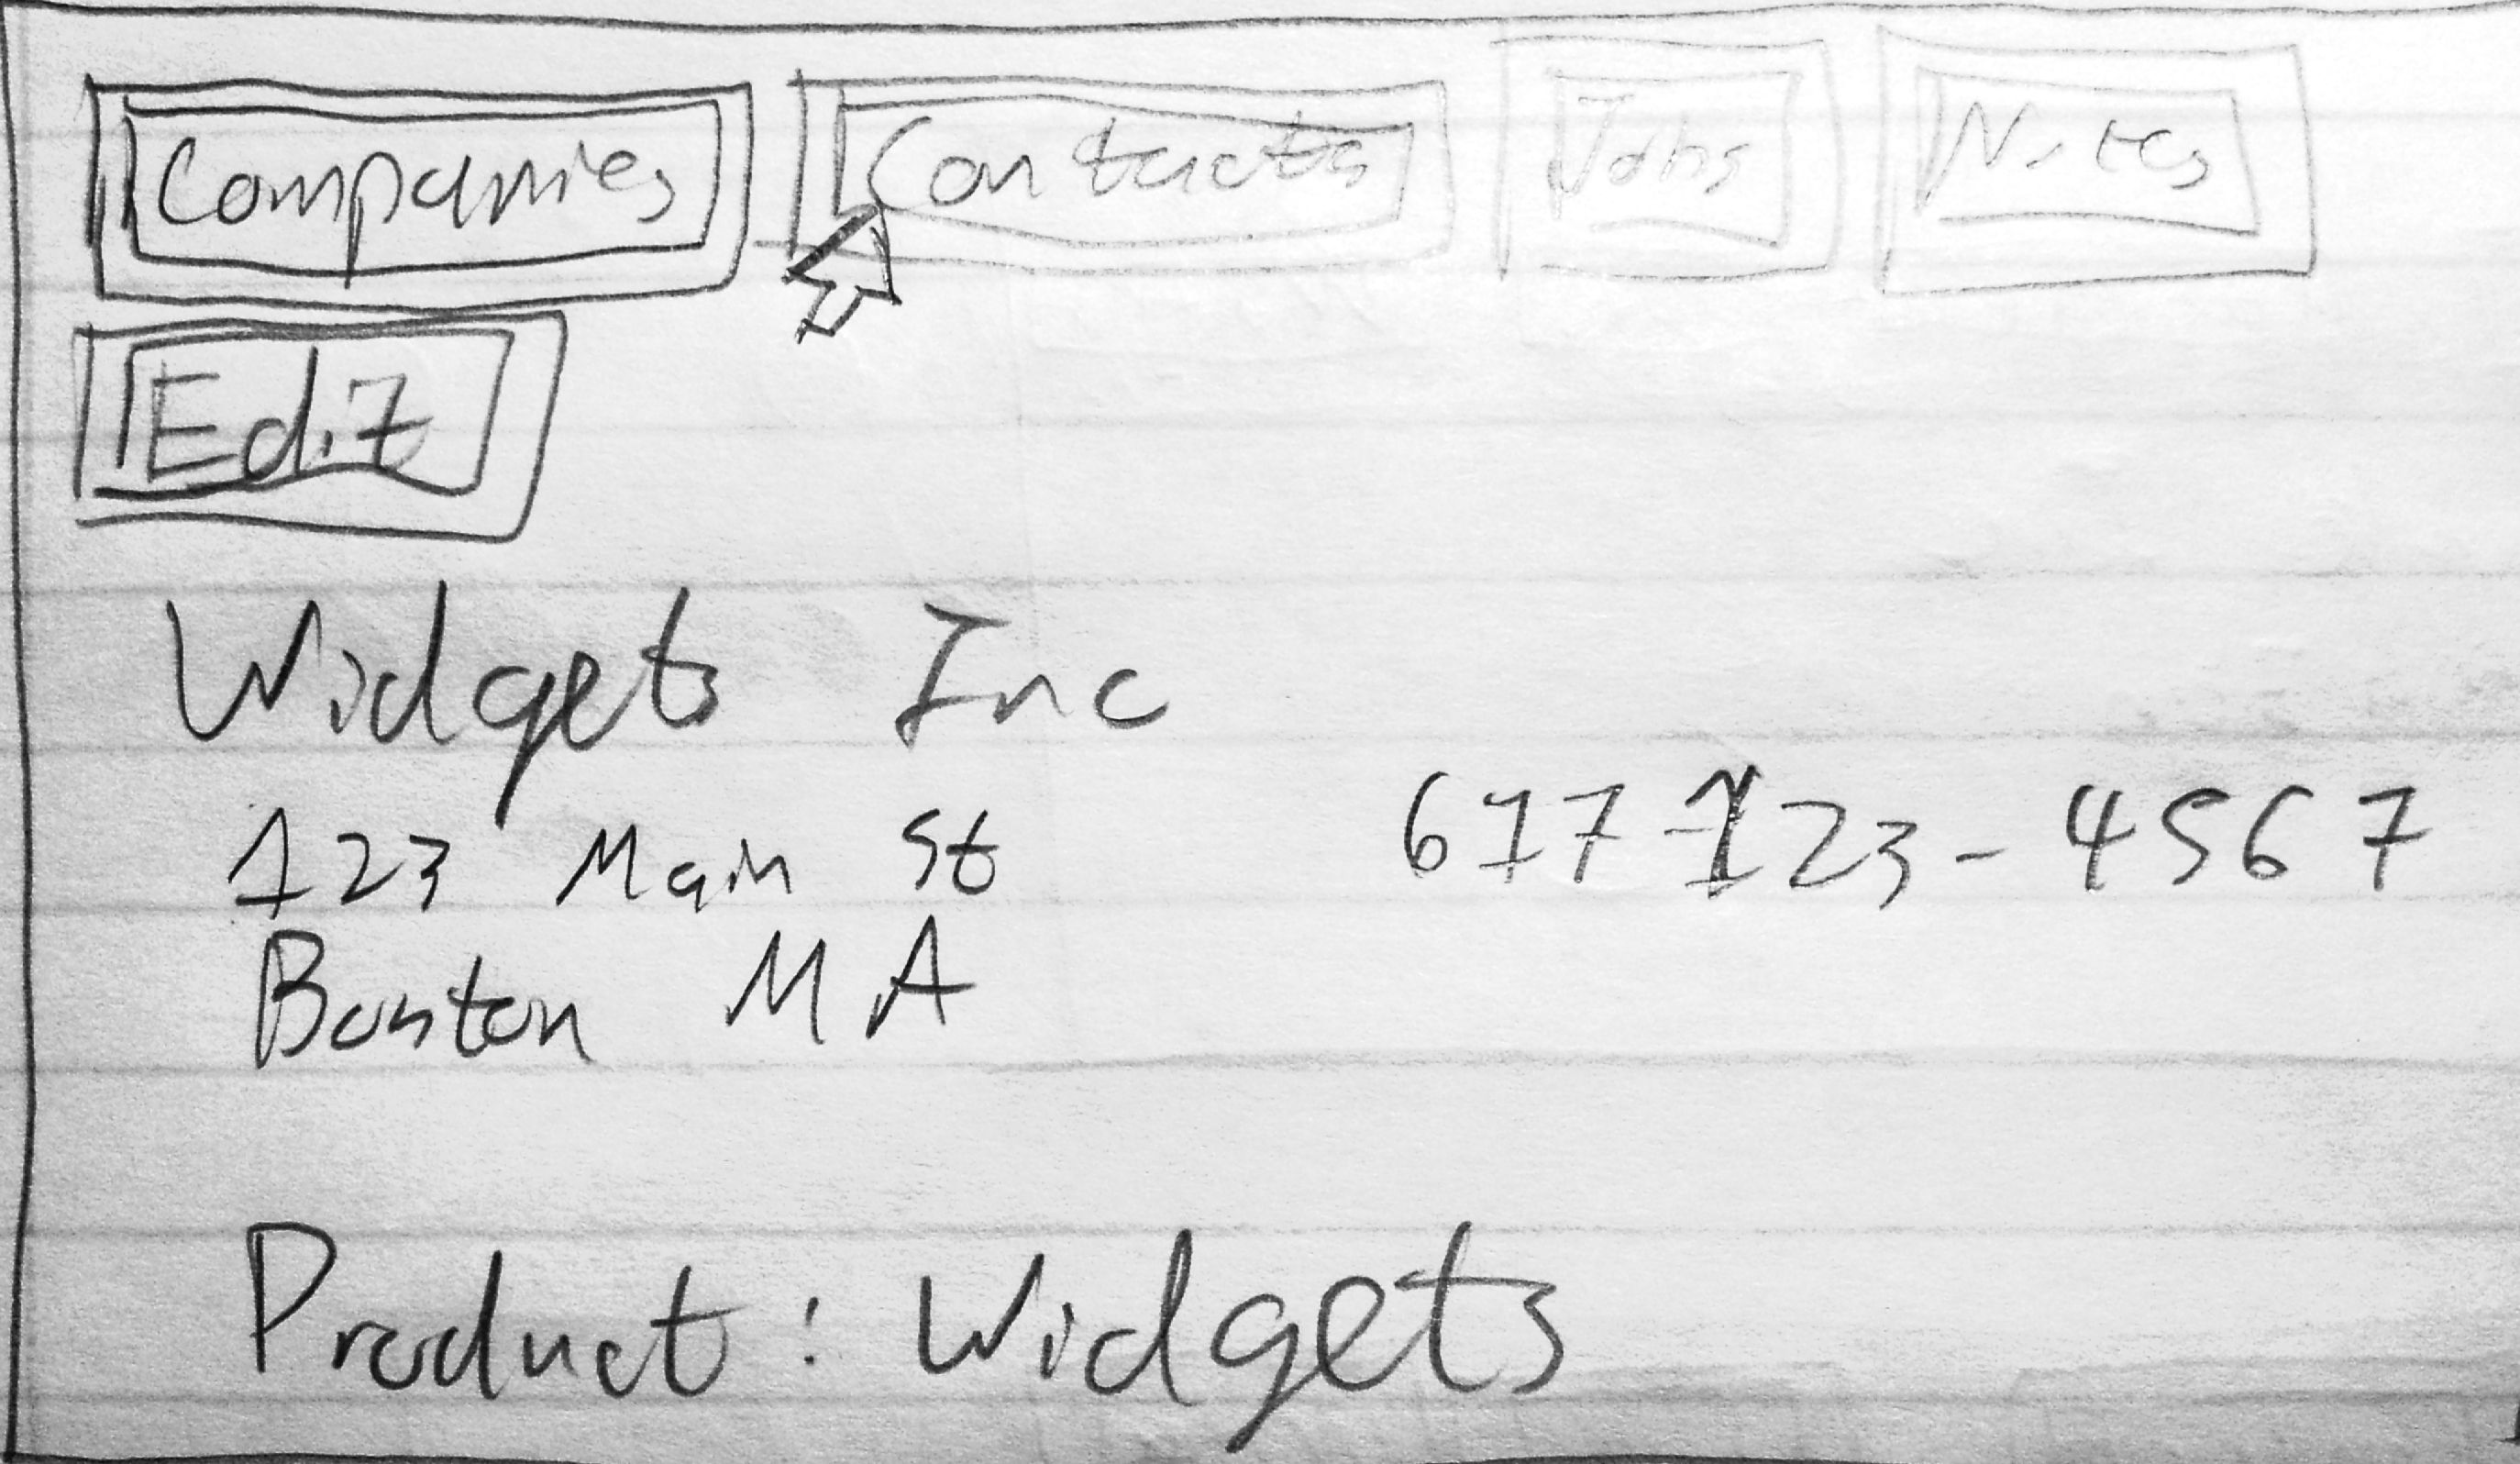
\includegraphics[width=\textwidth]{story_4.jpg}
\captionof{figure}{The company is saved, and we are shown the company information, but not editable.}
\end{minipage}


\vspace{.5cm}


\begin{minipage}[t]{.4\linewidth}
\centering
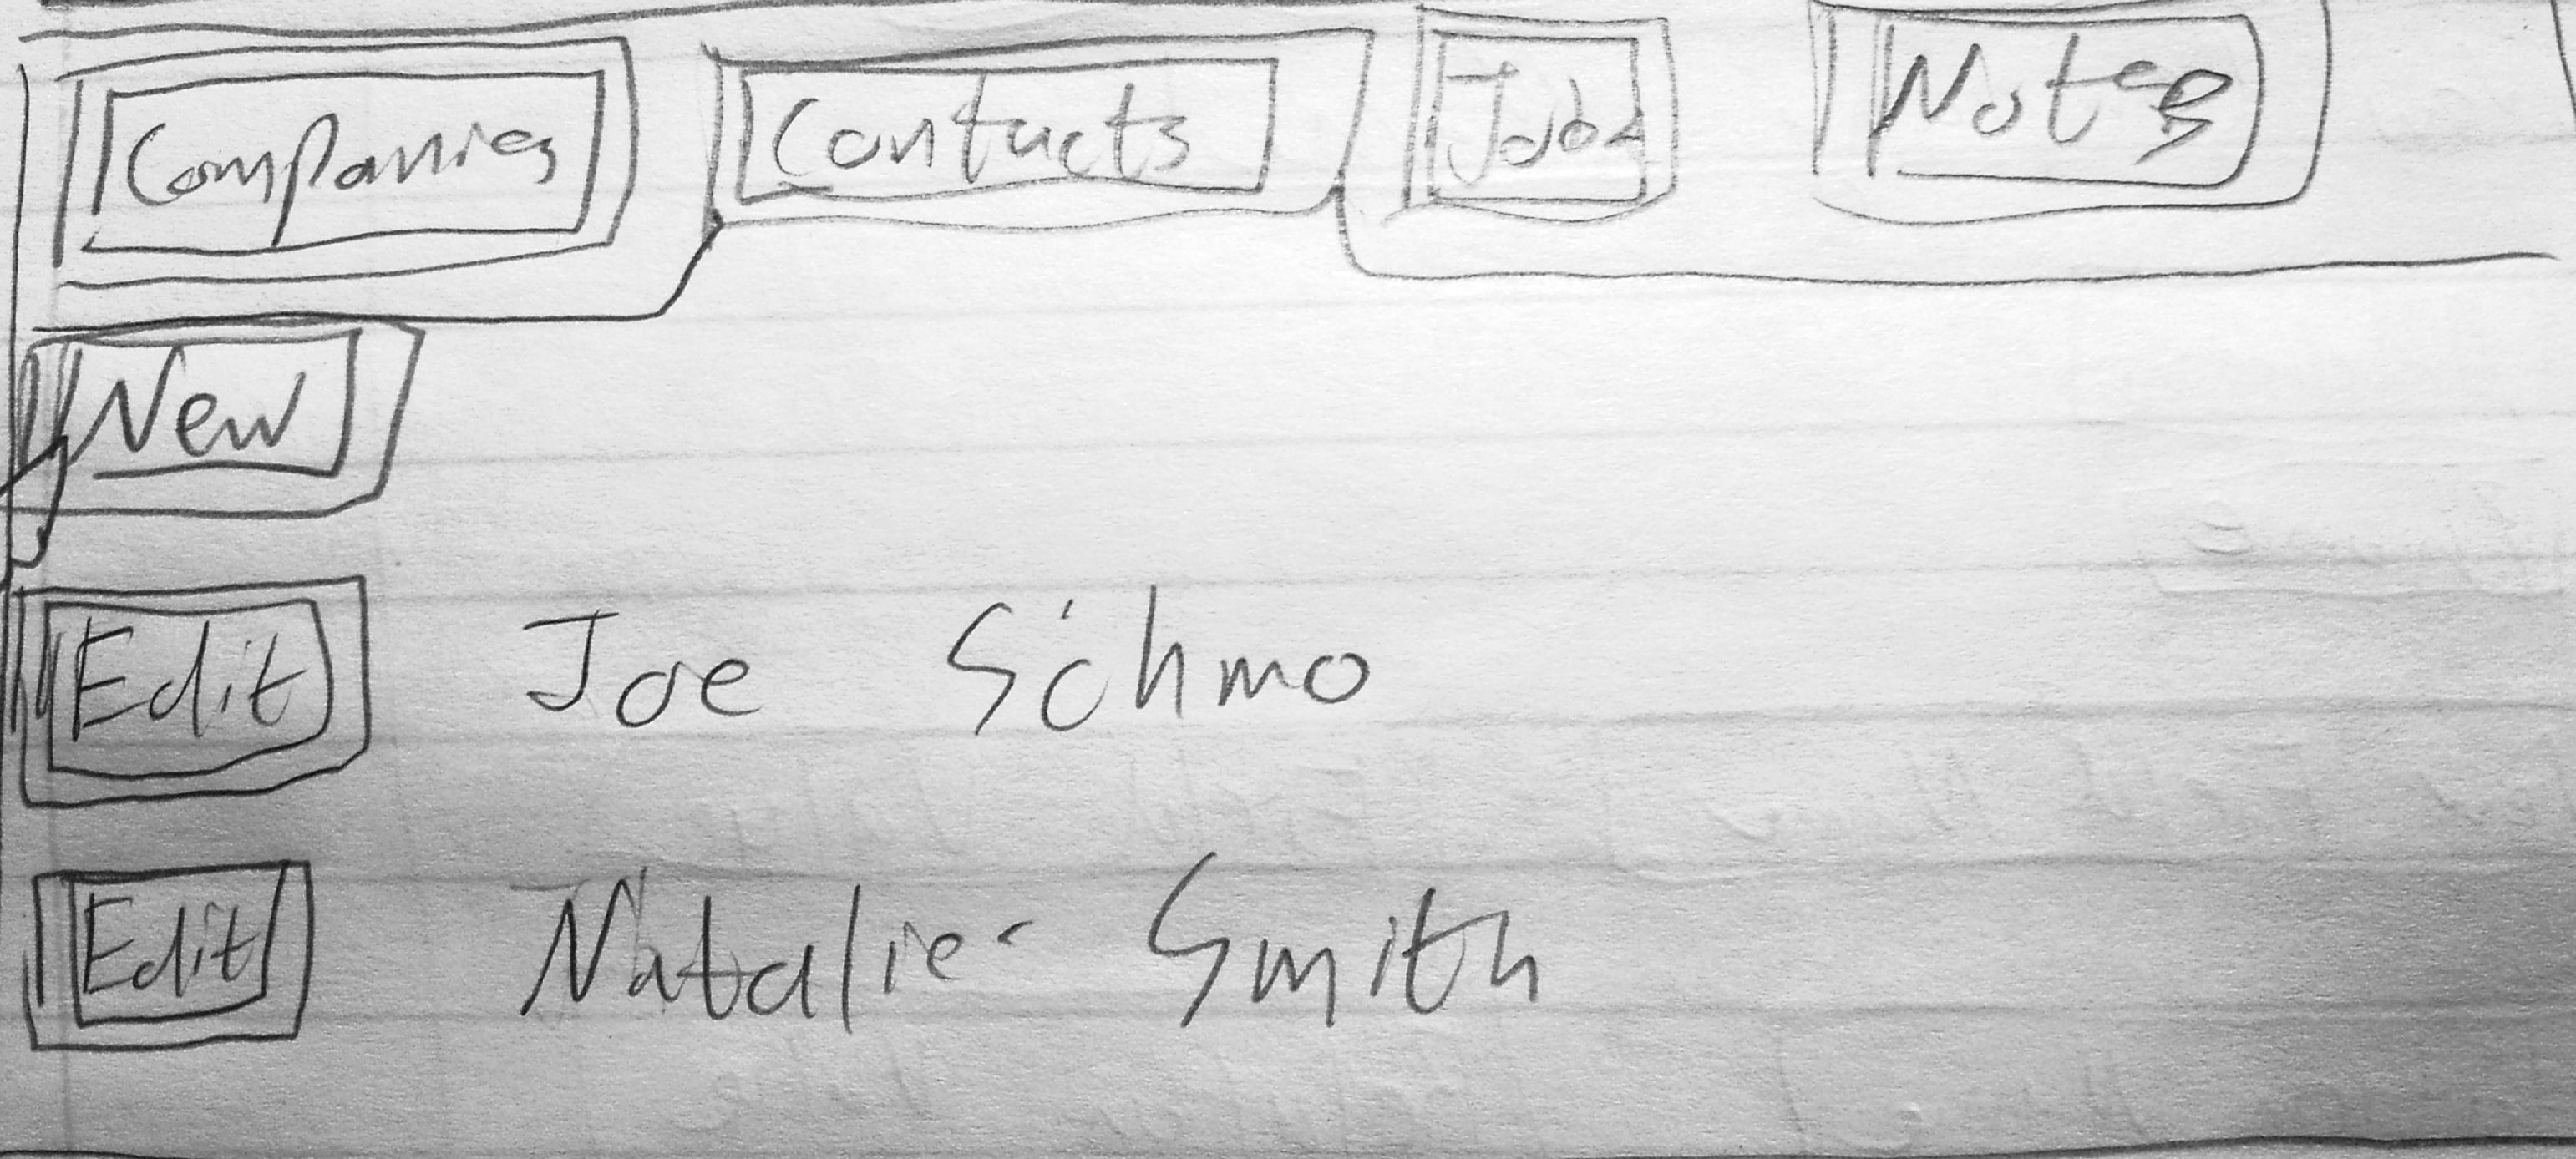
\includegraphics[width=\textwidth]{story_5.jpg}
\captionof{figure}{Now we are viewing the contact list, about to click on the "New" contact button.}
\end{minipage}
\hspace{.5cm}
\begin{minipage}[t]{.4\linewidth}
\centering
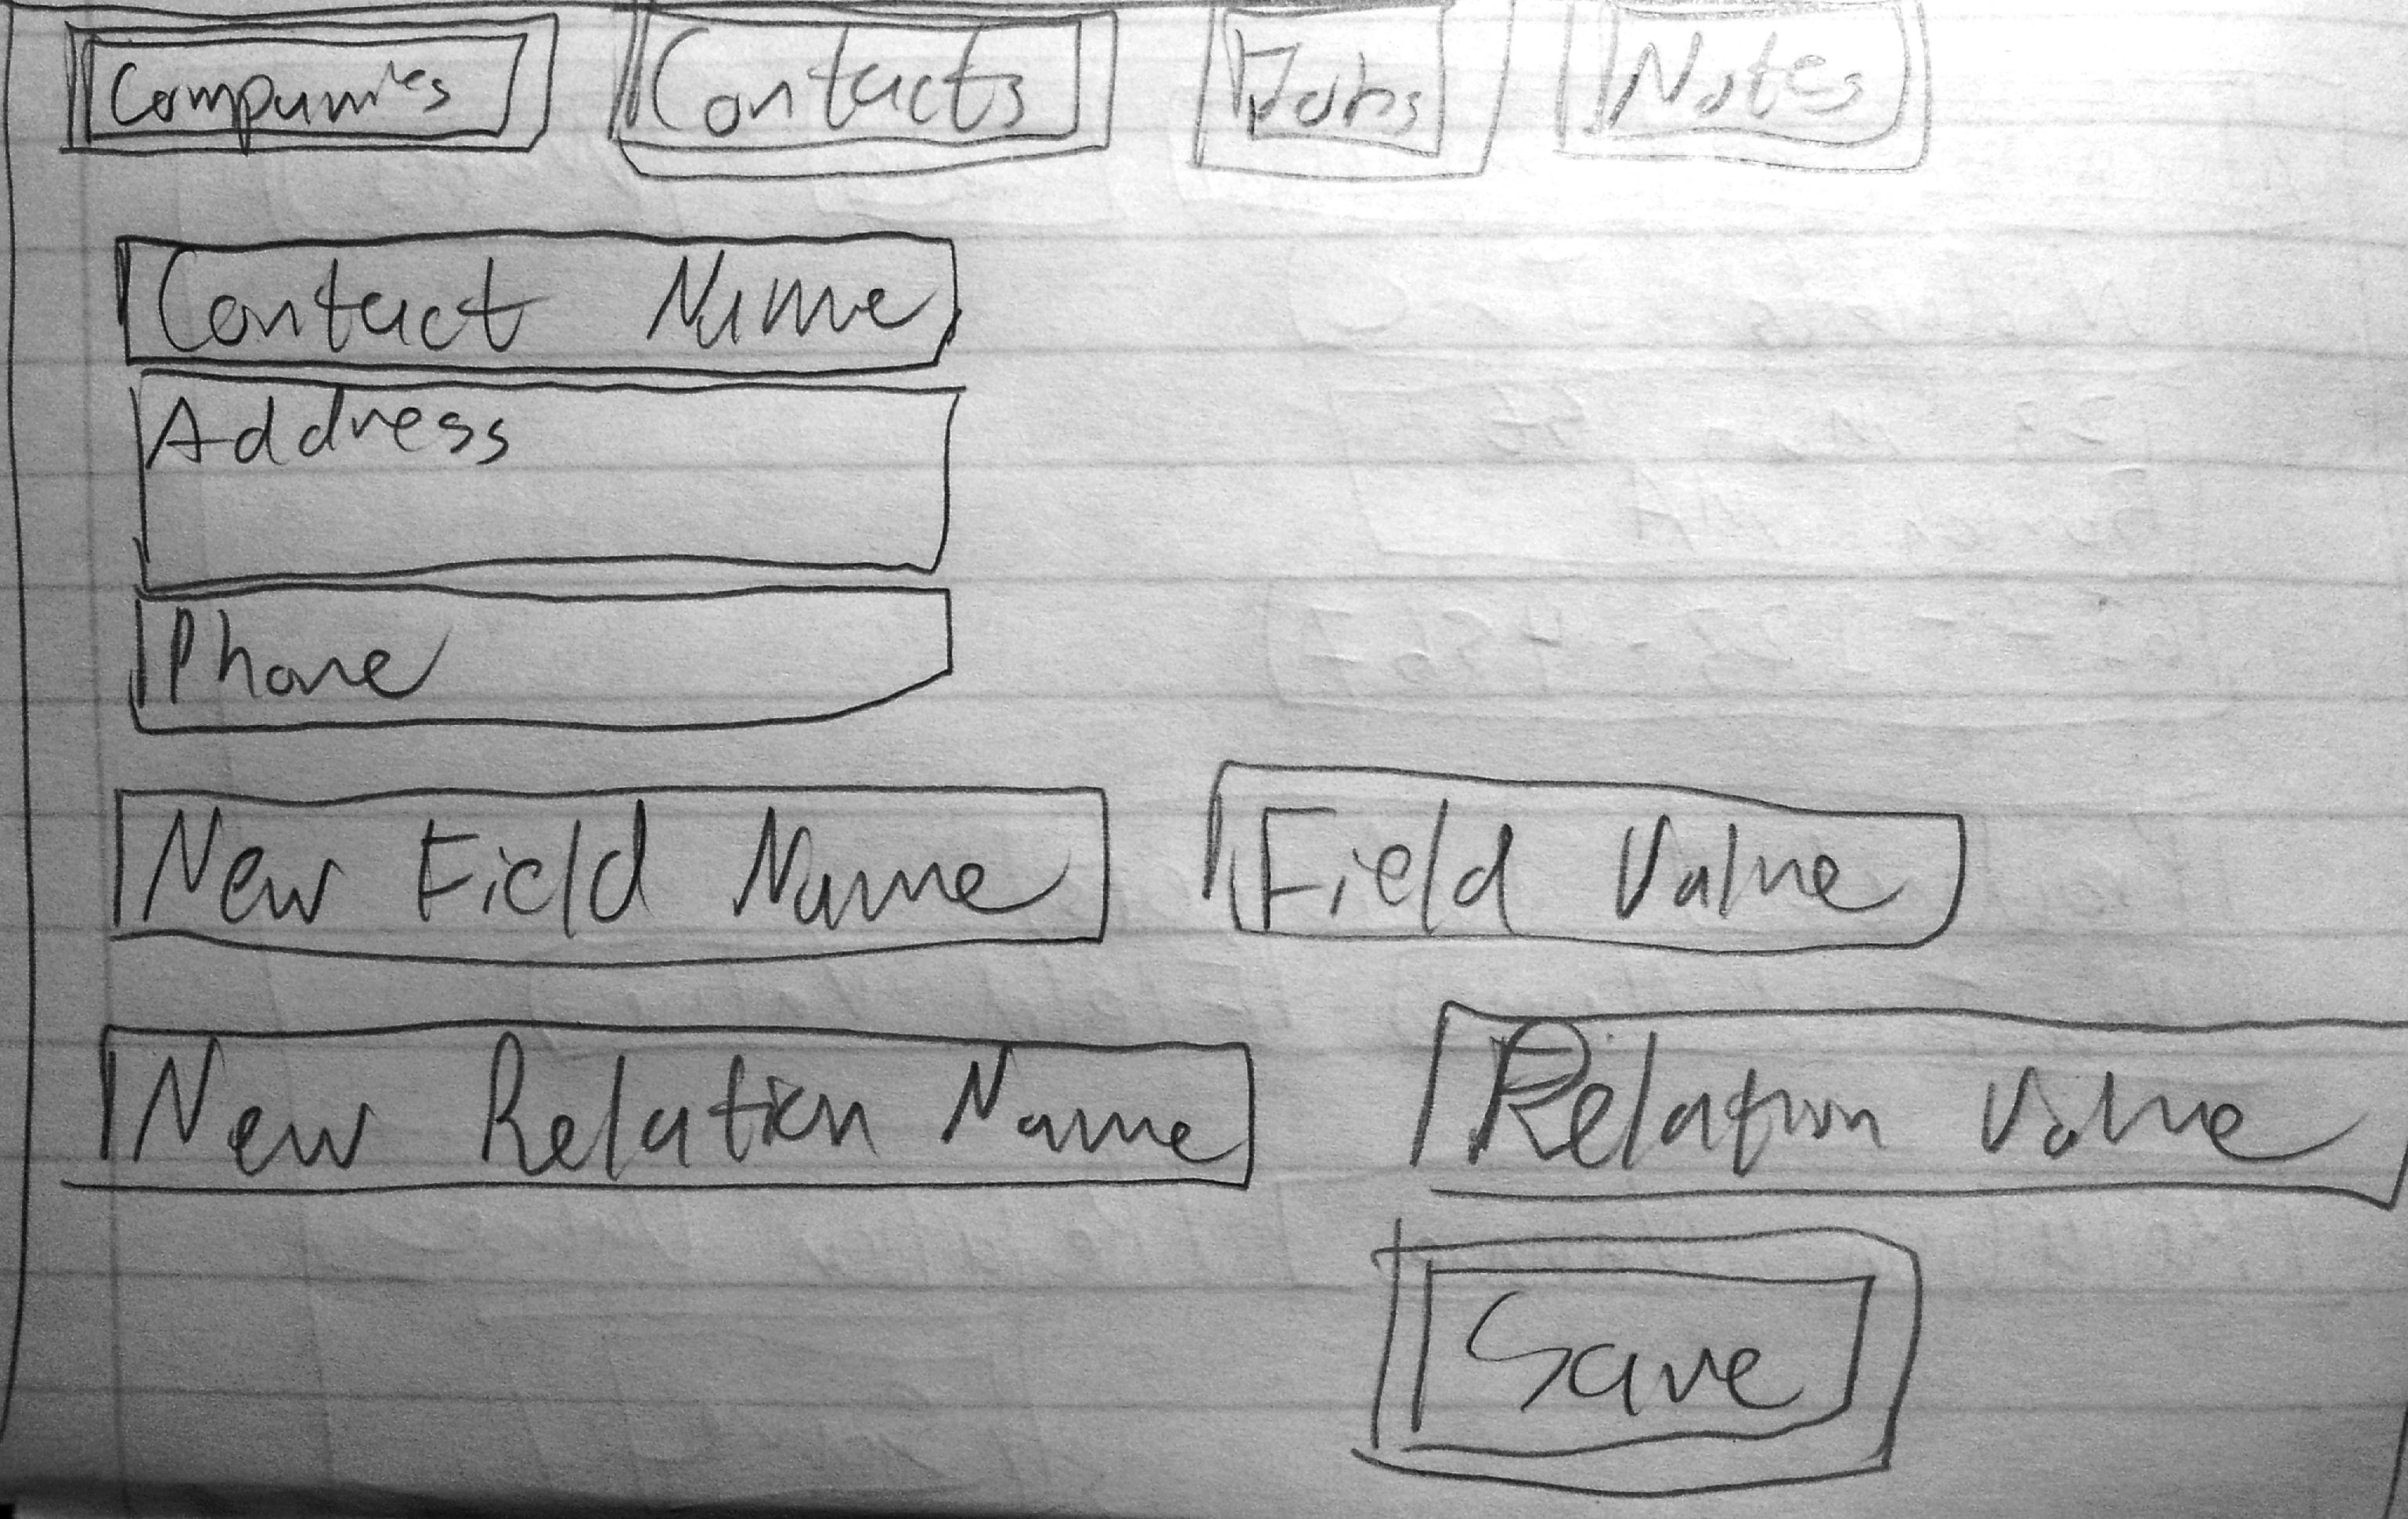
\includegraphics[width=\textwidth]{story_6.jpg}
\captionof{figure}{This is the new contact form, ready to be populated.}
\end{minipage}


\begin{minipage}[t]{.4\linewidth}
\centering
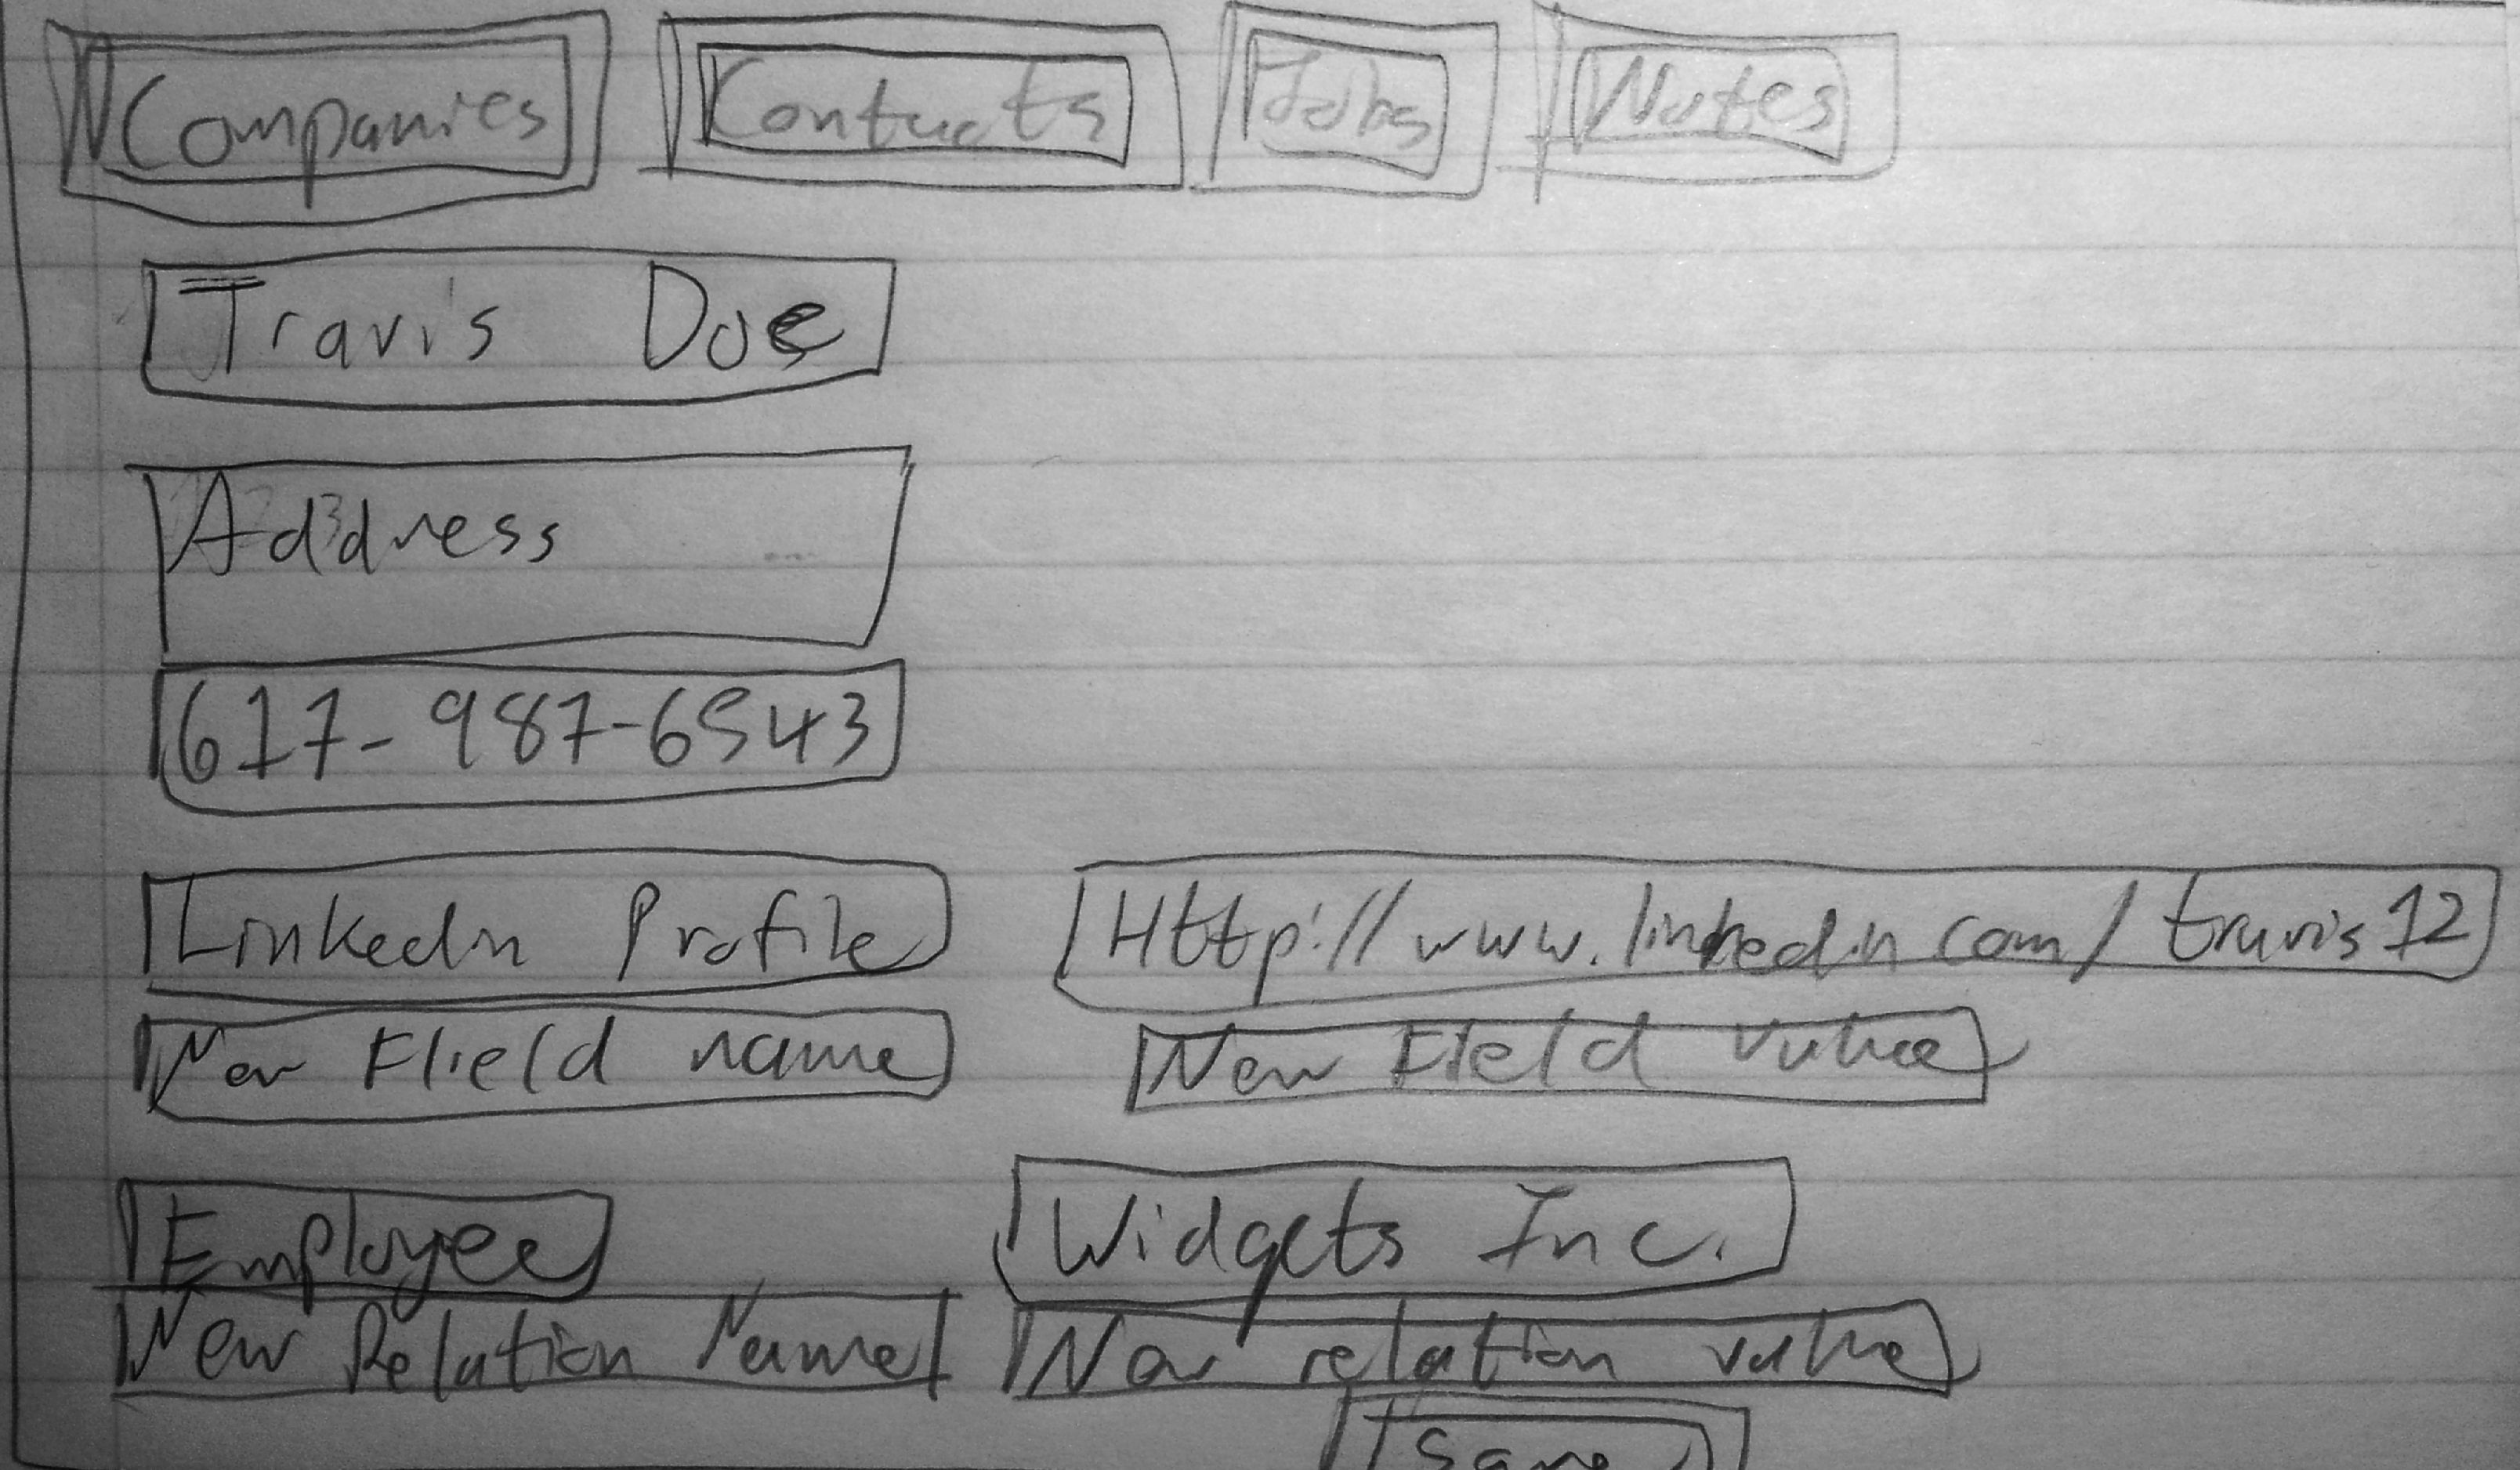
\includegraphics[width=\textwidth]{story_7.jpg}
\captionof{figure}{The contact is populated.  Notice both a custom field ("Linkedin profile") and a relation to the "Widgets Inc." company.}
\end{minipage}
\hspace{.5cm}
\begin{minipage}[t]{.4\linewidth}
\centering
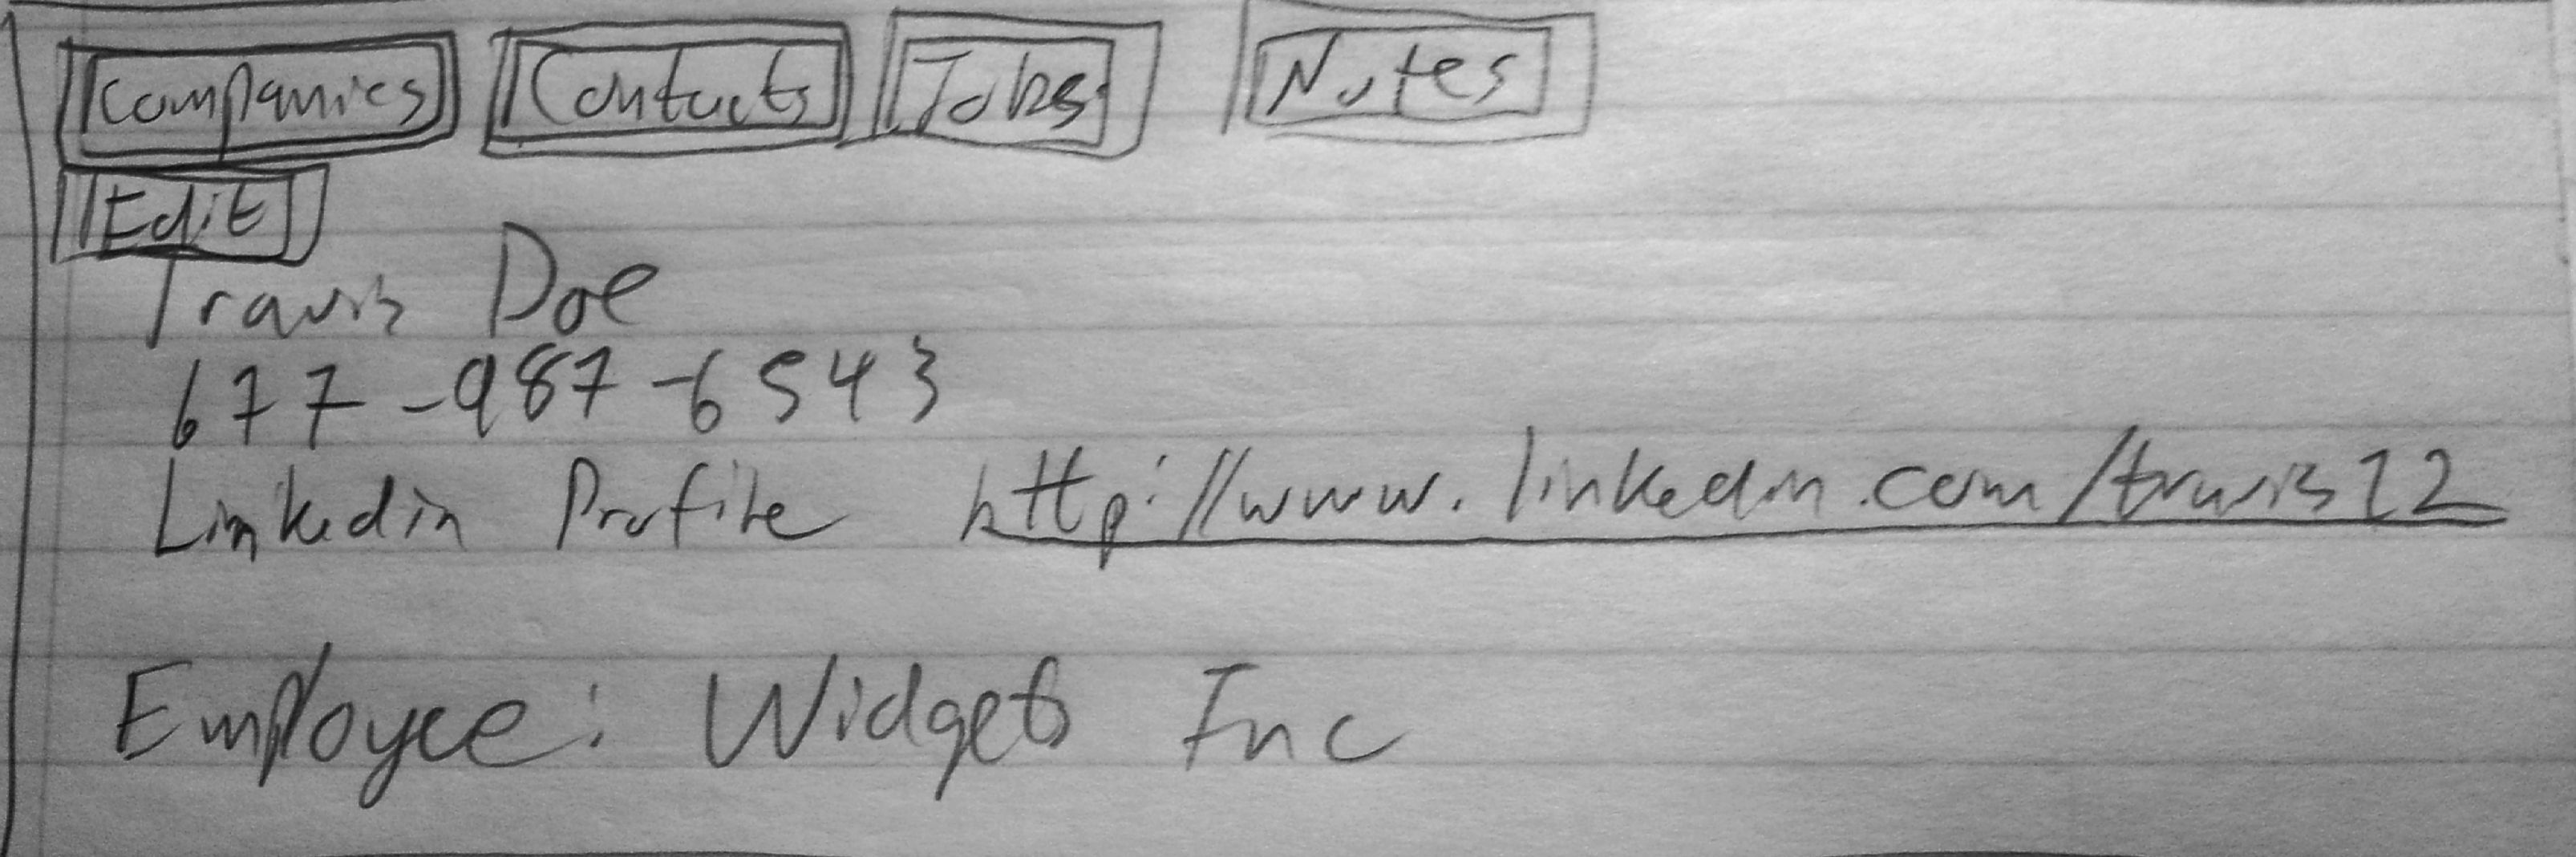
\includegraphics[width=\textwidth]{story_8.jpg}
\captionof{figure}{We click save, and are brought to the contact page for viewing, not editing.  Notice that since we did not provide an address, it does not appear here.}
\end{minipage}

\end{figure}

\section{User Documentation}

Hello, and welcome to \emph{Job Tracker 34,000 \texttrademark \textcopyright}, your one stop for all of your job hunting and networking needs.

\hfill

This system is easy and fun to use!  To record some new information, simply start by clicking on the type of thing you would like to add at the top of the page.  This will bring you to a list of the companies, people, jobs or notes that you have already recorded.  To add a new one, click the "New" button just below the category buttons.  Then, fill in information on the form that appears.

\hfill

If you want to edit an entry that you've entered in the past, start by navigating to the correct category page, just as before, finding the entry you want to edit on the list, and pressing the enter button.  Then, just as before, fill out the form with your new information.

\hfill

\emph{Job Tracker 34,000 \texttrademark \textcopyright}'s strength comes in two forms.  Firstly, when you're editing or creating a new entry, you can add any sort of information you want by creating a custom field.  This can be anything from a like to someone's linkedin profile to their favorite food.  Secondly, you can like different objects together, so you can record which company someone works at, or who you contact is for the job you're pursuing.

\hfill

Speaking of pursing jobs, let's go through how that process might work.  You find a company you like, so you create a company entry for it.  Then, you find a job you want to apply to, so you make a job entry for that position, linking it to the company it's at.  When you send you resume off for that job, make a note related to the job, so you don't forget that they have your resume.  If you hear back, make a 'contact' entry for the person who reaches out to you, and make notes recording what you've told them and what they've told you.

\hfill

Hopefully it can make your job hunt faster, easier, and more organized, with the help of \emph{Job Tracker 34,000 \texttrademark \textcopyright}!


\section{Task-Command Analysis}

\subsection{Inserting new object, tabbing between fields}

\begin{tabular}[H]{|p{5cm} | p{10cm}|}
\hline
Description & Action \\
\hline
Clicking to object list screen & hand movement across device \newline mouse click \\
Clicking new object button & hand movement across device \newline mouse click \\
Filling in fields &  hand movement from mouse to keyboard \newline keyboard presses \\
Clicking save & hand movement from keyboard to mouse \newline hand movement across device \newline mouse click \\
\hline
\end{tabular}

\vspace{.25cm}

\begin{tabular}[H]{|p{10cm}|p{2cm}|}
\hline
Action & Total \\
\hline
button press & 4 \\
hand movement across device or screen & 3 \\
hand movement between screen and other part of device & 2 \\
\hline
\end{tabular}

\subsection{Inserting new object, clicking between fields}

\begin{tabular}[H]{|p{5cm} | p{10cm}|}
\hline
Description & Action \\
\hline
Clicking to object list screen & hand movement across device \newline mouse click \\
Clicking new object button & hand movement across device \newline mouse click \\
Clicking and filling in field &  hand movement across device \newline mouse click \newline hand movement from mouse to keyboard \newline keyboard presses \newline hand movement from keyboard to mouse   \\
Clicking save & hand movement across device \newline mouse click \\
\hline
\end{tabular}

\vspace{.25cm}

\begin{tabular}[H]{|p{10cm}|p{2cm}|}
\hline
Action & Total \\
\hline
button press & 3 + 2 * num fields\\
hand movement across device or screen & 3 + 1 * num fields\\
hand movement between screen and other part of device & num fields\\
\hline
\end{tabular}

\subsection{Editing Object}

\begin{tabular}[H]{|p{5cm} | p{10cm}|}
\hline
Description & Action \\
\hline
Clicking to object list screen & hand movement across device \newline mouse click \\
Clicking new object button & hand movement across device \newline mouse click \\
Filling in fields &  hand movement from mouse to keyboard \newline keyboard presses \\
Clicking save & hand movement from keyboard to mouse \newline hand movement across device \newline mouse click \\
\hline
\end{tabular}

\vspace{.25cm}

\begin{tabular}[H]{|p{10cm}|p{2cm}|}
\hline
Action & Total \\
\hline
button press & 4 \\
hand movement across device or screen & 3 \\
hand movement between screen and other part of device & 2 \\
\hline
\end{tabular}

\subsection{Adding relation to Object}

\begin{tabular}[H]{|p{5cm} | p{10cm}|}
\hline
Description & Action \\
\hline
Clicking to object list screen & hand movement across device \newline mouse click \\
Clicking object's edit button & hand movement across device \newline mouse click \\
Filling in relation name &  hand movement across device \newline hand movement from mouse to keyboard \newline keyboard presses \\
Filling in relation value & hand movement from keyboard to mouse \newline hand movement across device \newline mouse click \\
Clicking save & hand movement across device \newline mouse click \\
\hline
\end{tabular}

\vspace{.25cm}

\begin{tabular}[H]{|p{10cm}|p{2cm}|}
\hline
Action & Total \\
\hline
button press & 5 \\
hand movement across device or screen & 4 \\
hand movement between screen and other part of device & 2 \\
\hline
\end{tabular}

\hfill

This is a relatively simple set of procedures, and a generally simple system overall.  I do no think that this paper analysis reveals any glaring problems with the current UI design.


\end{document}












































